%-----------------------------------------------
% Template para criação de resumos de projectos/dissertação
% jlopes AT fe.up.pt,   Fri Jul  3 11:08:59 2009
%-----------------------------------------------

\documentclass[9pt,a4paper]{extarticle}

%% English version: comment first, uncomment second
%\usepackage[portuguese]{babel}  % Portuguese
\usepackage[english]{babel}     % English
\usepackage{graphicx}           % images .png or .pdf w/ pdflatex OR .eps w/ latex
\usepackage{times}              % use Times type-1 fonts
\usepackage[utf8]{inputenc}     % 8 bits using UTF-8
\usepackage{url}                % URLs
\usepackage{multicol}           % twocolumn, etc
\usepackage{float}              % improve figures & tables floating
\usepackage[tableposition=top]{caption} % captions
%% English version: comment first (maybe)
%\usepackage{indentfirst}        % portuguese standard for paragraphs
%\usepackage{parskip}

%% page layout
\usepackage[a4paper,margin=30mm,noheadfoot]{geometry}

%% space between columns
\columnsep 12mm

%% headers & footers
\pagestyle{empty}

%% figure & table caption
\captionsetup{figurename=Fig.,tablename=Tab.,labelsep=endash,font=bf,skip=.5\baselineskip}

%% heading
\makeatletter
\renewcommand*{\@seccntformat}[1]{%
  \csname the#1\endcsname.\quad
}
\makeatother

%% avoid widows and orphans
\clubpenalty=300
\widowpenalty=300

\begin{document}

\title{\vspace*{-8mm}\textbf{\textsc{Remote, direct-manipulation
interaction for multi-user, web-based
public display applications}}}
\author{\emph{Maria João Barreira}\\[2mm]
\small{Projecto/Dissertação realizado sob a orientação da \emph{Prof.\ Maria Teresa Galvão}}\\
\small{no \emph{CITAR}}}
\date{}
\maketitle
%no page number 
\thispagestyle{empty}

\vspace*{-4mm}\noindent\rule{\textwidth}{0.4pt}\vspace*{4mm}

\begin{multicols}{2}

\section{Motivação}\label{sec:motiva}

Nowadays, the number of the public displays is increasing. It is usual to find them in public stations, waiting rooms and crowded places. 
However, most of them are only used with the purpose to advertise a product or a service preventing the interaction with the displays.

This scenario can be changed with recent developments in technology. This provide to users, an interaction with public displays, based on direct manipulation by their mobile device.

\section{Main Goals}\label{sec:goals}

This project has a challenging side. It encourages us to search some solutions in order to develop web applications for multi-users, based on direct-manipulation paradigm. 
In the end, the user must interact with applications by their own mobile device. 

The main goals of this project are:
\begin{itemize}
\item to develop and to validate an architecture that allows an interaction based on direct-manipulation;
\item to implement some applications examples which controls were created by the developed framework;
\item to test with the final users the framework and the applications.
\end{itemize}

\section{Developed Solution}\label{sec:work}

To achieve the defined goals, the solution is composed by three different components. In image ~\ref{fig:componentes}, we can see the server, the application that would be in a public display and the final user, the client.

\begin{figure}[H]
\centerline{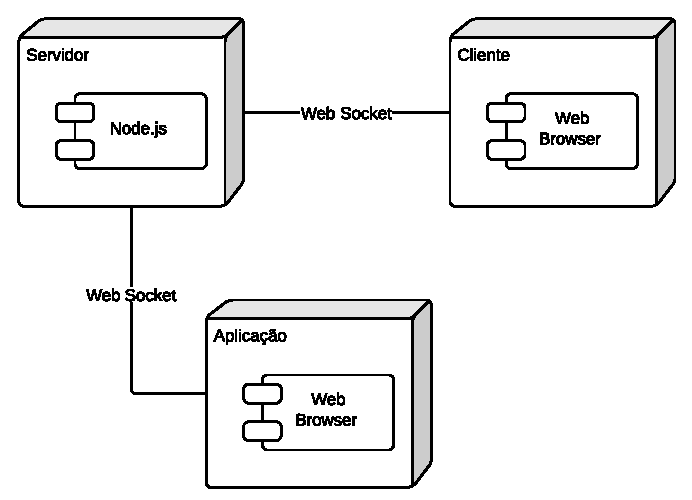
\includegraphics[scale=.5]{Components}}
\caption{Components of Solution}  
\label{fig:componentes}
\end{figure}

\subsection{Used Technologies}\label{sec:lingua}

During the development of all project we had to make some choices related to technologies used.

On the server side we used node.js. It is a scalable technology that enables you to rapidly build network applications that are lightning fast and highly concurrent.

To allows the communication between the server or user and the application we chose the Socket.io  library with the web sockets protocol.

We also applied to another libraries such as Prototype.js and Swipeable. The first one allows the manipulation of classes and objects based in classes. The second made easier the recognition of the swipe movements.

Beyond the referred technologies, all the project was developed based on JavaScript, HTML and CSS.

\subsection{Developed Framework} 

To make easier the development of applications to public displays, it was develop a framework to facilitate the creation of controls to the respective applications.
The framework allows the use of three different controls that can be used in several applications.
The programmer can choose which control is better according to the functionalities. His options are:

\begin{itemize}
\item \textbf{Joystick}: the directional arrows;
\item \textbf{Input Text}: a box of input text;
\item \textbf{Swipe}: to given an answer to the touches in display.
\end{itemize}

\subsection{Implemented Example}

As example, it was implemented the classic game Snake.

There is a QR code in the public display to allows the connection between the user device and the application. The QR code is always visible to let a new user has access to the game.

The user's device must be connected to the Internet and also have an application to read the QR code.

After this it is possible to enjoy the game and to use all of the defined controls.

First of all he needs to put his name using the input text widget. Only after that he can choose between joystick and swipe widget to control the snake during the game.

To change the control, according to his preferences, the user only needs to press the widget button that he wants to use.

In a public application for multi-users, it is important to explain how to distinguish the users.

In this particular case, we use the color of the respective snake to write in the display the name of the users with their scores, to make easier the recognition of the players.

\section{Conclusions}\label{sec:conclui}

In conclusion, not everything that we initially planned was effectively developed. However the main goals were accomplished.

A new framework was created to make easier the creation of the controls for interactive public applications as well as the implementation of a practical example.

In the end, it was also possible to make some tests with three students. They had to appeal to the functionalities of the framework to create the controls for the chosen application.

%%English version: comment first, uncomment second
%\bibliographystyle{unsrt-pt}  % numeric, unsorted refs
%\bibliographystyle{unsrt}  % numeric, unsorted refs
\bibliography{refs}

\end{multicols}

\end{document}
